\documentclass{article}
\usepackage{amsmath}
\usepackage{tikz}
\usetikzlibrary{arrows.meta,positioning,calc}

\begin{document}

\begin{figure}[h]
\centering
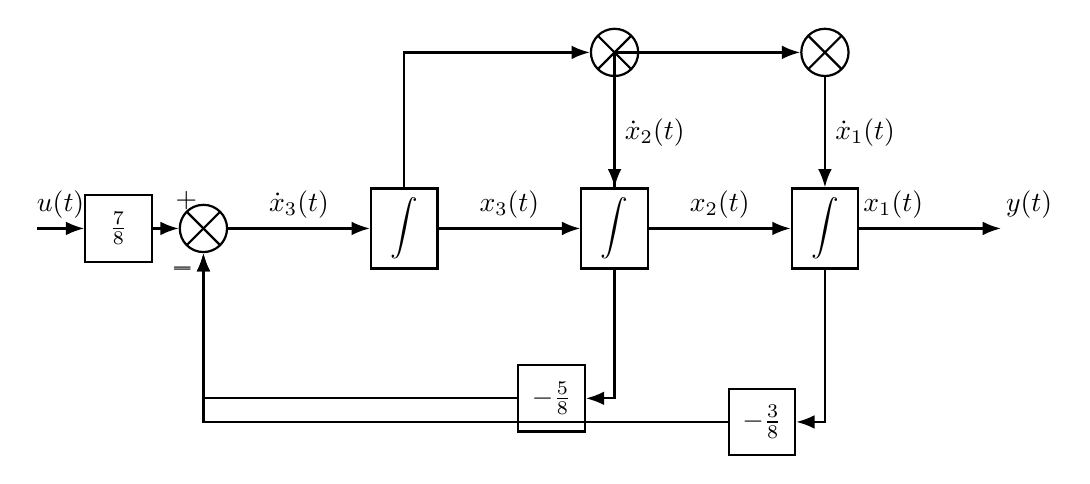
\begin{tikzpicture}[>=Latex, thick, node distance=2cm]

  % Styles
  \tikzset{
    block/.style={draw, rectangle, minimum height=2.4em, minimum width=2.4em, align=center},
    sum/.style={draw, circle, inner sep=0pt, minimum size=6mm, path picture={
        \draw (path picture bounding box.north west) -- (path picture bounding box.south east);
        \draw (path picture bounding box.north east) -- (path picture bounding box.south west);
      }},
    input/.style={coordinate},
    output/.style={coordinate}
  }

  % Main summing node for x3dot
  \node[input] (u) {};
  \node[sum, right=1.8cm of u] (sum3) {};

  % Integrator chain: x3 -> x2 -> x1
  \node[block, right=1.8cm of sum3] (int3) {$\displaystyle\int$};
  \node[block, right=1.8cm of int3] (int2) {$\displaystyle\int$};
  \node[block, right=1.8cm of int2] (int1) {$\displaystyle\int$};
  \node[output, right=1.8cm of int1] (y) {};

  % Chain labels
  \draw[->] (sum3) -- node[above] {$\dot x_3(t)$} (int3);
  \draw[->] (int3) -- node[above] {$x_3(t)$} (int2);
  \draw[->] (int2) -- node[above] {$x_2(t)$} (int1);
  \draw[->] (int1) -- node[above] {\quad\quad $x_1(t) \quad\quad\quad y(t)$} (y);

  % Summing node for x2dot = x3
  \node[sum, above=1.4cm of int2] (sum2) {};
  \draw[->] (int3) |- (sum2);
  \draw[->] (sum2) -- node[right] {$\dot x_2(t)$} (int2);

  % Summing node for x1dot = x2
  \node[sum, above=1.4cm of int1] (sum1) {};
  \draw[->] (int2) |- (sum1);
  \draw[->] (sum1) -- node[right] {$\dot x_1(t)$} (int1);

  % Feedback gains for x1 and x2 into main sum (x3dot)
  \node[block, below=1.5cm of int1, xshift=-0.8cm] (g_x1) {$-\frac{3}{8}$};
  \node[block, below=1.2cm of int2, xshift=-0.8cm] (g_x2) {$-\frac{5}{8}$};

  \draw[->] (int1.south) |- (g_x1);
  \draw[->] (g_x1) -| node[pos=0.95, left] {$-$} (sum3);

  \draw[->] (int2.south) |- (g_x2);
  \draw[->] (g_x2) -| node[pos=0.95, left] {$-$} (sum3);

  % Input u with gain 7/8 into main sum
  \node[block, right=0.6cm of u] (g_u) {$\frac{7}{8}$};
  \draw[->] (u) -- node[above] {$u(t)$} (g_u);
  \draw[->] (g_u) -- (sum3);
  \node[above=1mm] at ($(g_u)!0.8!(sum3)$) {$+$};

\end{tikzpicture}
\caption{State–space block diagram (only internal states $x_1,x_2,x_3$ and input $u$).}
\end{figure}

\end{document}